% !TeX root = ../../thesis.tex

\section{\acf{PI}}

\TODO{me}

\subsection{\acs{UEFI}/\acs{PI} Firmware Images}

\cite[Vol. 3, Section 2]{pi-spec} defines the firmware storage design.
A Firmware Image is stored in one or more non\-/volatile physical storage devices called \acp{FD}, they are most commonly flash devices \cite[Vol. 3, Section 2.1]{pi-spec}.
Flash often offers the ability to restrtict read and write properties differently depending on the storage region \cite[Vol. 3, Section 2.1.1]{pi-spec}.
\ac{UEFI} variables may reside in a region that remains read- and writable during the whole operation of a system, whereas the code storage may only be writable during the initial \ac{PI} phases.
Firmware images might be split over multiple physical \acp{FD}, but may also be inturn be logically be split into \acp{FV}.
\acp{FV} are comparable to hard drive volumes as they also are formatted with a file system, usually the \ac{PI} \ac{FFS} format defined in \cite[Vol. 3, Section 2.2]{pi-spec}.
The \ac{PI} \ac{FFS} is a flat file system consisting of a single list of files without any directory structure.
Parsing the volume is done by iterating over all files one by one.
Files contain code or data in the form of sections.
Sections split a file in discrete parts with the type of a section dictating its content.
File types impose restrictions on which types of sections a file may contain or not.
The full list of file types defined in the \ac{PI} specification can be seen in \autoref{tab:file-types}.
File sections are organized in trees, with encapsulating as well as leaf sections.
Together with the file section type \code{EFI\_SECTION\_FIRMWARE\_VOLUME\_IMAGE} which contains an entire \ac{PI} \ac{FV} image, this makes up for the \ac{FFS}'s lack of a directory structure.
The full list of section types can be seen in \autoref{tab:file-section-types}.

\autoref{fig:ovmf-in-uefitool} shows a firmware image opened in \program{UEFITool}, an editor for firmware images conforming to the \ac{PI} specification \cite{uefitool}.
The cursor is on the executable section of a \acs{DXE} driver.


\begin{figure}[htb]%
    \centering%
    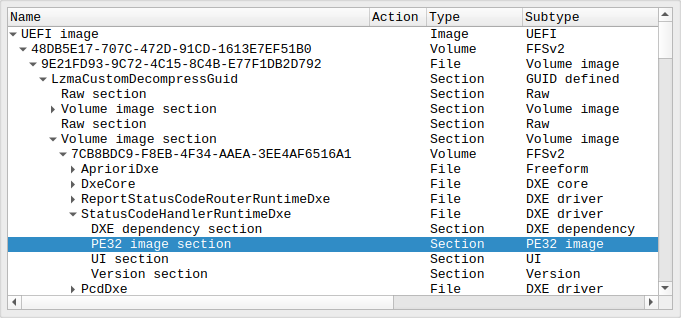
\includegraphics[width=\textwidth]{pi/ovfm_uefitool.png}%
    \caption{\ac{OVMF} opened in \program{UEFITool}}%
    \label{fig:ovmf-in-uefitool}%
\end{figure}


\subsection{\acs{PI} Architecture Firmware Phases}

The \ac{PI} Architecture defines distinct phases.
focus will be on dxe and transient system load
\autoref{fig:pi-phases}



\begin{figure}[htb]%
    \centering%
    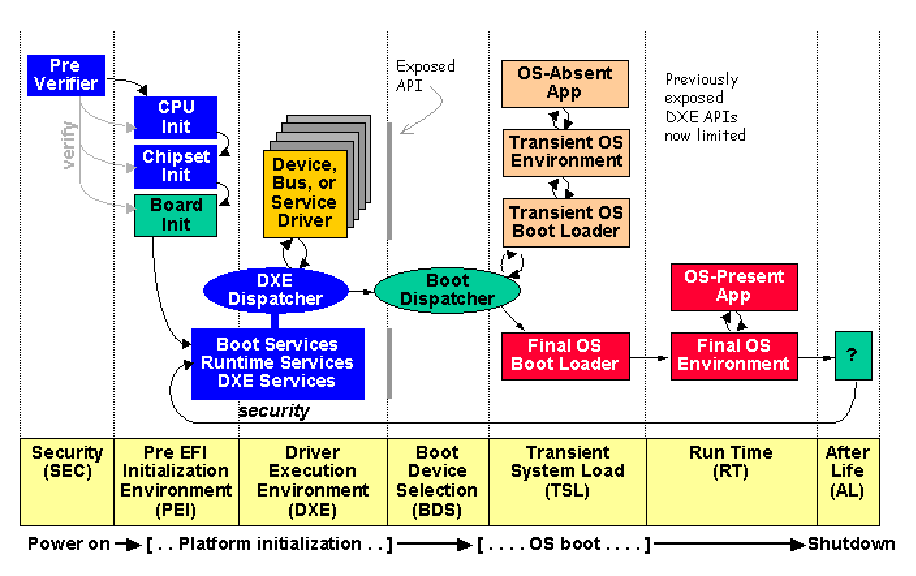
\includegraphics[width=\textwidth]{pi/pi_phases}%
    \caption{\ac{PI} Architecture Firmware Phases \cite[Figure 2-1]{pi-spec}}%
    \label{fig:pi-phases}%
\end{figure}


\subsubsection{\acf{SEC}}
% % Since the CPU doesn't know about UEFI or BIOS the initial step is exactly the same, it starts in 16-bit real mode and fetches it's first instruction from `CS = 0xF000` and `IP = 0xFFF0` but instead of shifting `CS` left by four bits and adding `IP`, the `CS` base register is initialized to `0xFFFF'0000`. So the first instruction is fetched from the physical address `0xFFFF'FFF0` (`0xFFFF'0000 + 0xFFF0`). The CS base address remains at this initial value until the CS selector register is loaded by software (e.g. far jump or call instruction)

% \begin{itemize}
%     \item Populates Reset Vector Data structure
%     \item Saves Built-in self-test (BIST) status
%     \item Enables protected mode (16 bit -> 32 bit)
%     \item Configures temporary RAM (not only limited in processor cache) by using MTRR to configure CAR.
% \end{itemize}


The \ac{SEC} phase is the first phase performed during platform initialization. Under its responsibilities fall handling all platform restart events, setting up temporary memory and establishing the system's root of trust. It serves as the foundation for all secure operations on which inductive security designs rely to build a chain of trust by having a module verify the integrity of its subsequent module. For this the \ac{SEC} phase may verify the integrity of the \ac{PEI} foundation before transfering execution to it. When it transfers execution, it also passes information about the current state of the system, including location and size of the temporary stack, \ac{RAM}, and \ac{BFV}. It can also optionally pass protocols for the \ac{PEI} phase to use.

\subsubsection{\acf{PEI}}

The \ac{PEI} phase configures the system to meet the minimum requirements for the \ac{DXE}.
Its job is the intialization of all system hardware requiring to be initialized beforehand, as well as the initialization of permanent memory, which is later described in \acp{HOB} to be passed off to the \ac{DXE} phase \cite[Vol. 1, 2.1]{pi-spec}.
The \ac{PEI} phase is architecturally a stripped down version of the \ac{DXE} phase, as it offers the same extensibility through modules supplied by the different \acp{OEM} responsible for the component initialization.
Even though the implementation of the \ac{PEI} phase is the most hardware dependent, the core functionality of the \ac{PEI} is common to all processor architectures and offered through the \ac{PEI} foundation \cite[Vol. 1, 2.2]{pi-spec}.
It is the module initially invoked by the \ac{SEC} phase and responsible of dispatching further \acp{PEIM} and offering a intermodule communication through the management of \acp{PPI} \cite[Vol. 1, 2.5]{pi-spec}.
The \ac{PEI} foundation implements a \ac{PEI} dispatcher, who iterates over \acp{PEIM} found in \acp{FV}, to evaluate their \acp{DEPEX}.
\acp{DEPEX} are logical combinations of \acp{PPI} that must be present before loading a \ac{PEIM}.
Loading \acp{PEIM} in turn enables them to install new \acp{PPI} and discover additional \acp{FV}, leading to previously unfullfilled \acp{DEPEX} now being fullfilled.
This process is repeated until no more \acp{PEIM} are able to be dispatched.
The foundation then invokes the \emph{\ac{DXE} IPL \ac{PPI}}, which loads the \ac{DXE} foundation into memory, to then transfer execution \cite[Vol. 1, 2.6]{pi-spec}.
The \ac{BFV} containing the \ac{PEI} foundation, initially discovered by the \ac{SEC} phase, and any additionally discovered \acp{FV} are also passed off to the \ac{DXE} in the form of \acp{HOB}.

While the \ac{PEI} phase has many architecturally required \acp{PPI} that modules have to implement, the \ac{PI} also defines optional \acp{PPI}.
One of which is the \emph{Security PPI}, it used to maintain the chain of trust by offering the chance for platform builders to authenticate or log \acp{PEIM} before they are executed \cite[Vol. 1, 6.3.6]{pi-spec}.


\subsubsection{\acf{DXE}}


The DXE Foundation produces a set of Boot, Runtime and DXE Services and exposes them through handle databases in the EFI System Table. It is designed to be completely portable, independent of processor, chipset and platform. The only dependent of the Hand-Off Blocks from the PEI phase, after these are processed the all prior phases can be unloaded.

% #### DXE Dispatcher

The DXE Dispatcher discovers DXE drivers within the Firmware Volume (FV) and executes them in the correct order, respecting their dependencies towards each other. The Firmware Volume file format allows the DXE driver images to be packaged with expressions about their dependencies. Since the DXE Drivers are PE/COFF images the dispatcher comes with an apropriate loader to load and execute the image format.

% #### DXE Drivers

% - Drivers that execute very early in the DXE phase
% - Drivers that comply with the UEFI Driver Model

The DXE Drivers are responsible for initializing the processor, chipset,
and platform components as well as providing software abstractions for console and
boot devices in the form of services.

dxe core/foundation
platform independent
is implementation of UEFI
UEFI Boot Services
UEFI Runtime Services
DXE Services

dxe dispatcher
discover drivers stored in firmware volumes and execute in proper order
apriori file optionally in FV or depex of driver
after dispatching all drivers in the dispatch queue hands control over to BDS

dxe drivers
init processor, chipset and platform
produce arichtectural protocols and \ac{I/O} abstractions for consoles and boot devices

% responsibilities
initializing the processor, chipset, and platform components
providing software abstractions for system services, console devices, and boot devices.

\TODO{DXE\_IMAGE sections and DEPEX section}

\subsubsection{\acf{BDS}}
The DXE Foundation will hand control to the BDS Architectural Protocol after all of the DXE drivers whose dependencies have been satisfied have been loaded and executed by the DXE Dispatcher.

% - Initializing console devices based on the ConIn, ConOut, and StdErr environment variables
% - Loading device drivers listed in the DriverOrder environment variables
% - Attempting to load and execute boot selections list from the BootOrder environment variables

During the BDS phase new Firmware Volumes (FV) might be discovered and control is once again handed to the DXE Dispatcher to load drivers found on these additional volumes.


DXE arichtectural protocol
one function entry
platform boot

attempts to connect boot devices required to load the os
discovers volumes containing new drivers
calls DXE dispatcher
doesnt return when successfully booting OS

UEFI itself only specifies the NVRAM variables used in selecting boot options
leaves the implementation of the menu system as value added implementation space \cite{uefi-spec}

\cite{pi-spec}

\begin{itemize}
    \item Initializing console devices
    \item Loading device drivers
    \item Attempting to load and execute boot selections
\end{itemize}

\subsubsection{\acf{TSL}}

The Transient System Load (TSL) is primarily the OS vendor provided boot loader. Both the TSL and the Runtime Services (RT) phases may allow access to persistent content, via UEFI drivers and UEFI applications. Drivers in this category include PCI Option ROMs.

This phase ends when an OS boot loader calls 'ExitBootServices()'.

boot and runtime services/driver
bootloader
\cite[Section 13.3]{uefi-spec}
\cite[Section 3.5.1.1]{uefi-spec}

ExitBootServices()

\subsubsection{\acf{RT}}
Boot service drivers have been unloaded and only runtime services are accessible.


runtime services/driver

\subsubsection{\acf{AL}}
The After Life (AL) phase consists of persistent UEFI drivers used for storing the state of the system during the OS orderly shutdown, sleep, hibernate or restart processes.

hibernation
sleep




% !TeX root = ../../thesis.tex

\subsection{Security}
\label{sec:uefi-pi:pi:security}

The \ac{PI} specification defines \acp{PPI} and \ac{DXE} protocols which can be used to validate images when loading them.
During the \ac{PEI} phase, the \emph{\ac{PEI} Guided Section Extraction \ac{PPI}} can be used to authenticate file sections, while the \emph{Security \ac{PPI}} implements the policy response to the authentication result.
The \ac{DXE} phase has counter parts in the form of the \emph{Guided Section Extraction Protocol} and the \emph{Security Architectural Protocol}.
The policy response may be the locking of flash upon authentication failure or attestation logging \cite[Vol. 2, Section 12.9.1]{pi-spec}.
It also has the architectural protocol \emph{Security2 Architectural Protocol}, which implements Secure Boot validation, \ac{TCG} measured boot, and User Identity policy for image loading.
The implementation of the boot service \code{LoadImage()} has to use these protocols in accordance to the rules defined in \cite[Vol. 2, Section 12.9.2]{pi-spec}.
The Security2 protocol is invoked on every loaded image, with the Security protocol being invoked afterwards on images loaded through the Firmware Volume Protocol.
When the Security2 protocol is not installed it uses the Security protocol regardless of the image's origin.

\subsubsection{Hardware Validated Boot}

Secure Boot relies on the firmware as its root of trust.
Hardware validated boot is able to shift the root of trust out of the firmware image into a smaller part in the hardware, in hopes to reduce the size of the attack vector.
This part performs validation of the \ac{IBB} before handing over execution to the firmware image \cite{tianocore-understanding-uefi-secure-boot-chain}.

\subsubsection{Firmware Protection}

The \ac{PI} specification defines an \emph{End of \acs{DXE} Event}, which indicates the introduction of third party software execution to the platform.
Up until this point it is assumed that the entire system software is under the control of the platform manufacturer.
Drivers may react to this event by locking critical system resources, using the \ac{SMM} related services \cite[Vol. 2, 5.1.2.1]{pi-spec}.
The \ac{SMM} is a secure execution environment, achieved by isolation from the rest of the system, through the \ac{CPU} \cite[Vol. 4, Section 1.3]{pi-spec}.
The \ac{PI} reference implementation also makes use of this event to lock the device that stores the firmware image \cite{tianocore-edk2-fmpdxe}.

